\documentclass[a4paper]{book}

\usepackage{graphicx,color}
\usepackage{amsmath}
\usepackage{fancyhdr}
\usepackage{makeidx}
\usepackage{alltt}
\usepackage{verbatim}
\usepackage{shortvrb}
\usepackage{verbatimfiles}
\usepackage{html}
\usepackage{xspace}
\usepackage{colortbl}

\usepackage{hyperref}
\usepackage{fancyvrb}

% --------------------------------------------------------------
% Make the sectioning a bit more fancy
% --------------------------------------------------------------

\usepackage{titlesec}

\titleformat{\chapter}[display]
{\normalfont\LARGE\filcenter\sffamily}
{}{1pc}
{\titlerule[1pt]%
\vspace{1pt}%
\titlerule
\vspace{2ex}\thechapter: }
[\vspace{2ex}\titlerule]

%\titleformat{\section}
%{\titlerule
%\vspace{.8ex}%
%\normalfont\itshape}
%{\thesection.}{.5em}{}

%\titleformat{\section}[frame]
%{\normalfont}
%{\filright
%\footnotesize
%\enspace\thesection\enspace}
%{8pt}{\Large\bfseries\filcenter}

\titleformat{\section}[frame]
{\normalfont}
{}{1ex}{\Large\thesection.\bfseries\filcenter}

\titleformat{\subsection}
{\normalfont\itshape\bfseries}
{\thesubsection.}{.5em}{}

% --------------------------------------------------------------
% Some formating stuff
% --------------------------------------------------------------

% I think it looks nicer if new paragraphs aren't indented
% as we have lots of whitespace anyway. just increase the 
% inter-paragraph space

\setlength{\parindent}{0pt} 
\addtolength{\parskip}{.5\baselineskip}


% --------------------------------------------------------------
% sundry shite
% --------------------------------------------------------------

\newcommand {\tbf}[1] {\textbf{#1}}
\newcommand {\tit}[1] {\textit{#1}}
\newcommand {\tmd}[1] {\textmd{#1}}
\newcommand {\trm}[1] {\textrm{#1}}
\newcommand {\tsc}[1] {\textsc{#1}}
\newcommand {\tsf}[1] {\textsf{#1}}
\newcommand {\tsl}[1] {\textsl{#1}}
\newcommand {\ttt}[1] {\texttt{#1}}
\newcommand {\tup}[1] {\textup{#1}}

\newcommand {\mbf}[1] {\mathbf{#1}}
\newcommand {\mmd}[1] {\mathmd{#1}}
\newcommand {\mrm}[1] {\mathrm{#1}}
\newcommand {\msc}[1] {\mathsc{#1}}
\newcommand {\msf}[1] {\mathsf{#1}}
\newcommand {\msl}[1] {\mathsl{#1}}
\newcommand {\mtt}[1] {\mathtt{#1}}
\newcommand {\mup}[1] {\mathup{#1}}

% spell things correctly  (like shite?)
\newenvironment{centre}{\begin{center}}{\end{center}}
\newenvironment{itemise}{\begin{itemize}}{\end{itemize}}

% define commands for describing functions, arguments and stuff
\newenvironment{funcDesc}{\vspace*{2mm}\begin{description}}{\end{description}\vspace*{2mm}}
\newenvironment{funcOpts}{\begin{description}}{\end{description}}
\newenvironment{funcExCode}{The code:\begin{alltt}\MakeShortVerb{\|}}{\DeleteShortVerb{\|}\end{alltt}}
\newenvironment{funcExOut}{Gives the output:\\}{}

\newcommand {\funcName}[1] {\ttt{#1}} % function name
\newcommand {\funcArg}[1] {\tit{#1}} % function argument
\newcommand {\reqArg}[1] {\tit{#1}} % required function argument
\newcommand {\optArg}[1] {\tit{#1}} % optional function argument
\newcommand {\defVal}[1] {\ttt{#1}} % default value of argument
\newcommand {\class} {\tbf{class\xspace}}
% option: first argument is option name, second argument is default
% value if any
\newcommand {\option}[1] {\item[\optArg{#1}: ]}  

\newcommand {\progName}[1] {\ttt{#1}} % external program name
\newcommand {\fileName}[1] {\tbf{\tit{#1}}} % file name



\usepackage[nottoc]{tocbibind}  
                                % allows the table of contents, bibliography
                                % and index to be added to the table of
                                % contents if desired, the option used
                                % here specifies that the table of
                                % contents is not to be added.
                                % tocbibind needs to be after natbib
                                % otherwise bits of it get trampled.

% --------------------------------------------------------------
% Code format within \Verb
% --------------------------------------------------------------

\definecolor{pycolor}{rgb}{0,0.4,0}

\DefineVerbatimEnvironment{python}{Verbatim}
{frame=leftline,framerule=.5mm,rulecolor=\color{pycolor},
formatcom=\color{pycolor}\small,fontshape=sl}

%\DefineShortVerb[formatcom=\color{dgreen}\small,fontshape=sl]{\|}

\RecustomVerbatimCommand{\Verb}{Verb}{formatcom=\color{pycolor}\small,fontshape=sl}

% --------------------------------------------------------------
% example environment
% --------------------------------------------------------------


%\newenvironment{example}{\begin{description}}{\end{description}}
%\newenvironment{example}{\begin{center}\begin{tabular}{|>{\columncolor[gray]{.9}}c|}\hline\\\begin{minipage}{.75\textwidth}}%
%{\end{minipage}\\\hline\end{tabular}\end{center}}

%\newenvironment{example}{\setlength{unitlength}{.8\textwidth}%
%\begin{center}%
%\begin{picture}(0,0)(-1,0)%
%\put(0,0){\line(1,0){.4\textwidth}\line(0,-1){1ex}}%
%\put(0,0){\line(-1,0){.4\textwidth}\line(0,-1){1ex}}%
%\end{picture}\\\begin{minipage}{.75\textwidth}}%
%{\end{minipage}\\x\end{center}}

\newenvironment{example}{%
\begin{center}%
%\makebox{\rule{.4\textwidth}{1pt}Hello\rule{.4\textwidth}{1pt}}\\[5mm]
\makebox[.8\textwidth]{\rule[-1ex]{1pt}{1ex}\hrulefill\ \raisebox{-1ex}{Example}\ \hrulefill\rule[-1ex]{1pt}{1ex}}\\[5mm]
\begin{minipage}{.75\textwidth}}%
{\end{minipage}\\[5mm]
\makebox[.8\textwidth]{\rule{1pt}{1ex}\hrulefill\rule{1pt}{1ex}}\end{center}}


% --------------------------------------------------------------
% Page layout
% --------------------------------------------------------------
% Page layout ... set for A4

\setlength{\topmargin}{-1.0 cm}
\setlength{\oddsidemargin}{0 cm}
\setlength{\evensidemargin}{0 cm}
\setlength{\textwidth}{18.5 cm}
\addtolength{\textwidth}{-\marginparsep}
\addtolength{\textwidth}{-\marginparwidth}
\setlength{\textheight}{26.5 cm}
\addtolength{\textheight}{-\footskip}

\pagestyle{fancyplain}
\renewcommand{\chaptermark}[1]{\markboth{Chapter \thechapter: #1}{}}
\renewcommand{\sectionmark}[1]{\markright{\thesection\ #1}}
\lhead[\fancyplain{}{\bfseries\thepage}]{\fancyplain{}{\bfseries\rightmark}}
\rhead[\fancyplain{}{\bfseries\leftmark}]{\fancyplain{}{\bfseries\thepage}}
\rfoot{}
\cfoot{}


% this code hacked from that of R Chandrasekhar from UWA
\newif\ifpdf
\ifx\pdfoutput\undefined
        \pdffalse    % we are not running pdfLaTeX
\else
        \pdfoutput=1 % we are running pdfLaTeX
        \pdftrue
\fi

\ifpdf
        \DeclareGraphicsExtensions{.pdf}  % this command defined in graphicx
        \pdfcompresslevel=9  % 0: no compression, 9: highest compression
                             % or, set compress_level 9 in file pdftex.cfg
\else
        \DeclareGraphicsExtensions{.eps}
\fi

\begin{document}

\begin{titlepage}
\begin{center}
\vspace*{3cm}
\LARGE

\includegraphics{figs/logo}\\[4cm]

{\Huge \emph{Pyscript}}\\[1cm]
\emph{Postscript Graphics with Python}\\[2cm]

v 0.6\\[2cm]

Alexei Gilchrist\\
Paul Cochrane
\end{center}
\end{titlepage}

\frontmatter

\tableofcontents

\mainmatter

%==========================================================================
\chapter{Introduction}
\label{cha:introduction}


\section{Overview}

\Verb|Pyscript| is a python package for creating high-quality postscript
drawings.  It began from the frustration of trying to create some good figures
for publication that contained some abritrary \LaTeX{} expressions, and has
been largely inspired by \Verb|mpost|. What began as some quick-n-dirty hacks
has evolved into a really useful tool (after several rewrites). Essentially a
figure is scripted using python and some pre-defined objects such as
rectangles, lines, text etc. This approach allows for a precise placement of
all the components of a figure.

Some of the key features are
\begin{itemize}
\item All scripting is done in python, which is a high-level, easy to
  learn, well developed scripting language.
\item All the objects can be translated, scaled, rotated, \ldots in fact any
affine transformation.  
\item The plain text object is automatically kerned.
\item You can place abritrary \LaTeX{} expressions on your figures.
\item You can create your own objects, and develop a library of figure 
primitives. 
\item Output is publication quality.
\end{itemize}

\section{Conventions and Pitfalls}
\label{sec:conventions}

Just to be clear from the outset, some conventions follow, and some common
pitfalls to be aware of \ldots

\begin{itemize}
\item The co-ordinate system is as you learned at school in maths \ldots
  the $x$-axis extends to the right, the $y$-axis extends upwards. I know, 
  this is obvious, but a suprising number of graphics libraries invert the 
  $y$-axis.
\item Angles are in degrees and proceed clockwise from the top \ldots
  just like your clock.  Often, key points are labeled by the compass
  points: n, ne, e, se, s, sw, w, nw.
\item The default units are postscript points,
  $1\mathrm{cm}=28.346\mathrm{pp}$. For a figure, the default can
  easily be changed with the command
  \Verb|defaults.units=UNITS['cm']|. All of the examples in this manual are
  in \texttt{cm}.
\item In python, an integer divided by an integer is truncated to an
  integer, To avoid this use floating point numbers, e.g. \Verb|2/3 = 0|
  but \Verb|2/3. = 0.6666|.
\item Backslashes in strings have special significance, such as
  denoting newlines (\Verb|"\n"|). This can be frustrating for
  entering \LaTeX{} expresions. You can turn off this interpretation by
  using raw strings: just prepend an ``r'' to the string e.g.
  \Verb|g=r"$\alpha$"|
\end{itemize}


\section{Tutorial}
\label{sec:tutotial}

As a tutorial, we'll take a detailed look at the script that created the
following figure:
\begin{center}
  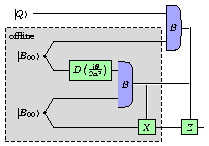
\includegraphics{figs/tutorial}
\end{center}
In the following script, we've interdispersed 
comments explaining what we're doing, the full script is available
with the other examples and is called \texttt{tutorial.py}.

First import the \Verb|pyscript| libraries, and we'll grab some objects
from \Verb|pyscript.lib.quantumcircuits| too. Most scripts would have
something like this at the beginning.
\begin{python}
from pyscript import *
from pyscript.lib.quantumcircuits import *
\end{python}
The default units are in postscript points. I prefer to use
\texttt{cm} so switch the units here. The default units are stored in
\Verb|defaults.units| which is just a number giving giving the
multiplying factor compared to postscript points. \Verb|UNITS| is a
dictionary of factors for some common units.
\begin{python}
defaults.units=UNITS['cm']
\end{python}
There's a bunch of \LaTeX{} macros I use often. Rather than defining
them each time they're needed, well define them in the \Verb|tex_head|
variable in \Verb|defaults|, which defines the start of the
environment where \emph{all} the \LaTeX{} is processed.
\begin{python}
defaults.tex_head=r"""
\documentclass{article}
\pagestyle{empty}
\usepackage{amsmath}

\newcommand{\ket}[1]{\mbox{$|#1\rangle$}}
\newcommand{\bra}[1]{\mbox{$\langle #1|$}}
\newcommand{\braket}[2]{\mbox{$\langle #1|#2\rangle$}}
\newcommand{\ketbra}[2]{\mbox{|#1$\rangle\langle #2|$}}
\newcommand{\op}[1]{\mbox{\boldmath $\hat{#1}$}}
\newcommand{\R}[3]{%
\renewcommand{\arraystretch}{.5}
$\begin{array}{@{}c@{}}{#1}\\{#2}\end{array}{#3}$
\renewcommand{\arraystretch}{1}
}
\begin{document}
"""
\end{python}
Now, define the colors of some objects here to make it easy to change
them everywhere in the figure later if we need to. There are a whole
variety of ways to specify a color, we'll use RGB values here.
\begin{python}
blue=Color(.65,.65,1)
green=Color(.65,1,.65)
\end{python}
There's a component of the figure we'll use several times, so for
convenience, define it here as a function which returns the object. 
A separate class would also be possible, but would involve more work.
We could also have created the object and used the \Verb|copy()| method
to make duplicates, but that would be clumsy.
\begin{python}
def BellDet(c=P(0,0)):

    H=P(0,.8)
    W=P(.5,0)
\end{python}
\Verb|D| is a D-shaped path filled in with the blue color we defined earlier.
\begin{python}
    D=Path(c+H,
           C(c+H+W),
           c+W,
           C(c-H+W),
           c-H,bg=blue,
           )
\end{python}
Now return everything as a \Verb|Group|, which will then get treated as a unit 
in the rest of the figure.
\begin{python}
    return Group(
        Path(c-H,c+H,linewidth=2),
        D,
        TeX(r'$\mathcal{B}$',c=D.c)
        )
\end{python}
To create the big gray box, we've tweaked the parameters after
examining the results so that it looks nice. The dash specification is
straight from postscript.
\begin{python}
offline=Rectangle(height=4,width=5.5,e=P(3.5,1.5),
                  dash='[3 ] 0',bg=Color(.85))
\end{python}
Now render the figure! What about all the other bits of the figure?
Well, we'll render them on the fly since we don't need to refer to the
objects again. \Verb|render| is a function that can take a variable
number of arguments, we'll create some of the objects in the
actual function call.

Objects are rendered in the order that they appear in the \Verb|render()| 
call.  So, we'll put on the big gray box first, this way it'll appear to be 
behind everything else.
\begin{python}
render(
    offline,
    TeX('offline',nw=offline.nw+P(.1,-.1)),
\end{python}
Now draw the lines, and some dots. A rough sketch on a piece of paper
beforehand will really help in figuring out what the co-ordinates are
for what you want to draw. You can always tweak them later.
\begin{python}
    Path(P(5,0),P(-.3,0),P(-.6,.5),P(-.3,1),P(2,1)),
    Path(P(2,2),P(-.3,2),P(-.6,2.5),P(-.3,3),P(3.7,3)),
    Path(P(-1,4),P(3.7,4)),

    Dot(P(-.6,.5)),
    Dot(P(-.6,2.5)),
\end{python}
Now add a double line, notice how the central region of the line in
the figure is unbroken? Can you guess how it was done?
\begin{python}
    classicalpath(Path(P(2.1,1.5),P(4.5,1.5),P(4.5,0)),
                  Path(P(3,1.5),P(3,0)),
                  Path(P(3.8,3.5),P(4.5,3.5),P(4.5,1.5)),
                  ),
\end{python}
Use the function we defined earlier to add those large detectors to the figure.
\begin{python}
    BellDet(P(2,1.5)),
    BellDet(P(3.7,3.5)),
\end{python}
Add some boxed equations to the figure. This object is from the
\Verb|quantumcircuits| library, and will add a box around an
abritrary object.
\begin{python}
    Boxed(TeX(r'$D\left(\frac{i\theta}{2\alpha^2}\right)$'),c=P(1,2),bg=green),

    Boxed(TeX('$X$'),c=P(3,0),bg=green),
    Boxed(TeX('$Z$'),c=P(4.5,0),bg=green),
\end{python}
Finally, add some \LaTeX{} expressions (notice some of the macros we
defined earlier), and give the filename to write the postscript to.
N.B.  keywords, such as \Verb|file=|, have to go after parameters in a
function call.
\begin{python}
    TeX(r'$\ket{B_{00}}$',e=P(-.7,.5)),
    TeX(r'$\ket{B_{00}}$',e=P(-.7,2.5)),
    TeX(r'$\ket{Q}$',e=P(-1.1,4)),

    file="tutorial.eps",
    )
\end{python}

We're done. Sit back and admire the figure.
%==========================================================================
\chapter{How Do I ...?}
\label{cha:howto}

%--------------------------------------------------------------------------
\section{Aligning things}

\Verb|pyscript| has a rich structure for aligning objects. This ranges
from objects which have attributes which specify a particular point
such as the nw corner of the object to functions such as
\Verb|Align()| and \Verb|Distribute()| which will align and distribute a 
group of objects.

%--------------------------------------------------------------------------
\subsection{Using attributes}

Certain objects (mostly those subclassed from \Verb|Area|) have named points
on the object that can be read or set. \Verb|Area| defines the
following compass points located on a rectangle: ``n'', ``ne'',
``e'', ``se'', ``s'', ``sw'', ``w'', ``nw''. Also the center of the
area is given by ``c''. Reading one of these attributes will return
the value of that point, and setting one of
these attributes will move the object so that the named point lies
on the supplied one. For example, \Verb|obj1.c=obj2.c| will align the
centres of the two objects. The points returned are vectors from the origin 
and can be manipulated in the usual ways.
\begin{example}
  This will align the centre of \Verb|obj3| so that it lies half way
  between the centres of \Verb|obj1| and \Verb|obj2|:
  \Verb|obj3.c=(obj1.c+obj1.c)/2.|.
\end{example}

The main thing to keep in mind is that the named point is for the
\emph{objects} coordinate system. If a transformation is applied to
the object, it will also be applied to all the named points.
\begin{example}
  As the following example shows, the named point always stays the same 
  in the objects coordinate system (watch the dot).
\begin{python}
r=Rectangle(width=2,height=2)
g=Group()

for a in [0,20,40]:
    p=P(a/7.,0)
    r2=r.copy(c=p).rotate(a,p)
    g.append(r2,Dot(r2.nw))

render(g,file=...)
\end{python}
produces
\begin{center}
  \includegraphics[width=.25\textwidth]{figs/fig_position_eg1}
\end{center}
\end{example}

%--------------------------------------------------------------------------
\subsection{Understanding boundingboxes}

An objects boundingbox is a rectangle in the \emph{current} coordinate
system that completely contains the object. The bounding box for an object
can be obtained with the \Verb|bbox()| method. The bounding box is calculated
after all the co-ordinate transformations are applied to the objects.

Bounding boxes have the same named point as rectangles, but these are
read-only, and you can't apply transformations to bounding boxes.

\begin{example}
  A variation of the previous example, where we'll put a dot at the
  nw corner of the bounding box
\begin{python}
r=Rectangle(width=2,height=2)
g=Group()

for a in [0,20,40]:
    p=P(a/7.,0)
    r2=r.copy(c=p).rotate(a,p)
    g.append(r2,Dot(r2.bbox().nw))

render(g,file=...)
\end{python}
produces
\begin{center}
  \includegraphics[width=.25\textwidth]{figs/fig_position_eg2}
\end{center}
\end{example}


%--------------------------------------------------------------------------
\subsection{Using Align()}

%--------------------------------------------------------------------------
\subsection{Using Distribute()}

%--------------------------------------------------------------------------
\section{Trouble Shooting}

\subsection{\LaTeX Stuff}

One of the useful features of \pyscript{} is the ability to use \LaTeX.
The process is kind of complicated though so things can break. It helps
to know how it all works if you're going to find some of the subtle bugs,
so here's a synopsis:
\begin{enumerate}
\item You create some \LaTeX{} with the \Verb|TeX()| object (you are using
  raw strings arent you?).
\item \pyscript{} writes the text to a temporary file sandwiched
  between \Verb|defaults.tex_head| and \Verb|defaults.tex_tail|. 
\item \Verb|defaults.tex_command| is excecuted on the file
\item \Verb|dvips| is executed on the resulting DVI file.
\item \pyscript{} reads the BoundingBox comment and throws the rest away!
\item Finally, within \Verb|render| \emph{all} the \Verb|TeX()|
  objects are collected together. A temporary file with all the \LaTeX{}
  is generated with the individual objects delimited by postscript
  tags (inserted via specials) and pagebreaks.
\item As before, \Verb|defaults.tex_command| is executed (twice this
  time) on the file, followed by \Verb|dvips|.
\item The resulting code is parsed and divided up into sections on
  fonts and procedures, and the individual postscript code for each
  object. These are then used within the final document.
\end{enumerate}
The reason it's so complicated is for efficiency --- you don't want all the
header and font info for every single piece of \TeX{} you put on the page.

This is \emph{not} the way \LaTeX{} was designed to be used and it
shows --- you have to jump through a number of hoops to get it all to
work. The \Verb|defaults.tex_command| should have a
\Verb|-interaction=batchmode| flag or errors won't get picked up. For
the same reason, \emph{any} output from \Verb|dvips| is treated as an
error, so it needs a \emph{-q} flag. There are a number of tweaks that
have to be made to the postscript code so that it is viable and the
boundingboxes work \ldots

Despite all this it works suprisingly well. You can even include
figures in the \LaTeX{} code and input other files etc. Take care
though, use \Verb|\input| rather than \Verb|\include| as the latter
seems to invoke some weird things in \Verb|dvips| that result in the
postscript tags not getting placed in the file. Also, don't use a figure
or table environment --- they're floats \ldots think about it.

Right, that enough of a rant. The useful stuff:
\begin{itemize}
\item output from the commands goes to the log file --- you did look
  at it right?
\item For each \Verb|TeX| object the temporary file thats created is
  called \Verb|temp1.tex|.  \Verb|defaults.tex_command| and
  \Verb|dvips -E| execute on it to produce \Verb|temp1.eps|. All these
  should be valid files which you can examine. You can also run the
  commands by hand to see whats going on.
\item The final temp file with all the objects is \Verb|temp.tex|
  which ends up producing \Verb|temp.ps| which will have one object
  per page. Again you can examine these files by hand.
\end{itemize}

%--------------------------------------------------------------------------
\section{Transformations and Things}


%==========================================================================
\chapter{Pyscript Objects}
\label{cha:base-objects}

These are the basic \Verb|pyscript| objects and functions. At the
begining of each class there is a brief description of the structure
of the class showing the relevant methods and members. See also
figure~\ref{fig:classes} on page~\pageref{fig:classes} for an
indication of how the classes fit together.

%--------------------------------------------------------------------------
\section{Base Objects}

These are classes which add layers of functionality to pyscript objects.
Normally you wouldn't use these classes directly unless you're creating new 
pyscript objects. We'll decribe them here because they summarise what
you can do with pyscript objects.

%--------------------------------------------------------------------------
\subsection{PsObj()}
\label{sec:psobj}
\begin{python}
class PsObj(object):
    def __call__(self,**dict):
        Set a whole lot of attributes in one go

    def copy(self,**dict):
        return a copy of this object
        with listed attributes modified

    def __str__(self):
        return actual postscript string to generate object

    def body(self):
        subclasses should overide this for generating postscipt code

    def bbox(self):
        return objects bounding box
\end{python}

Base class of which most (all?) \Verb|pyscript| classes are subclass.

A list of parameters can be set when an object is created with
calls like \Verb|t=Text('Hello',font='Helvetica')|
or by calling the object like a function as in \Verb|t(sw=P(0,2))|.
The parameters are also available singly as attributes: \Verb|t.sw| etc.

Printing an object produces the actual postscript code.

Objects may be copied with the \Verb|copy()| function and new
parameters can be passed in as arguments eg \Verb|s = t.copy(sw=P(0,0))|.

%--------------------------------------------------------------------------
\subsection{AffineObj()}
\label{sec:affineobj}
\begin{python}
class AffineObj(PsObj):

    o=P(0,0)
    T=Matrix(1,0,0,1)

    def concat(self,t,p=None):
        concat matrix t to tranformation matrix
          t: a 2x2 Matrix dectribing Affine transformation
          p: the origin for the transformation
          return: reference to self

    def move(self,*args):
        translate object by a certain amount
          param args: amount to move by, can be given as
            - dx,dy
            - P
          return: reference to self

    def rotate(self,angle,p=None):
        rotate object, 
        the rotation is around p when supplied otherwise
        it's the objects origin
          angle: angle in degrees, clockwise
          p: point to rotate around (external co-ords)
          return: reference to self

    def scale(self,sx,sy,p=None):
        scale object size (towards objects origin or p)
          sx sy: scale factors for each axis
          p: point around which to scale
          return: reference to self

    def itoe(self,p_i):
        convert internal to external co-ords
          p_i: intrnal co-ordinate
          return: external co-ordinate
        
    def etoi(self,p_e):
        convert external to internal co-ords
          p_e: external co-ordinate
          return: internal co-ordinate
\end{python}

A base class for objects that should implement affine transformations
(such as scaling, rotating etc), this should apply to any object that
draws on the page.


%--------------------------------------------------------------------------
\subsection{Area()}
\label{sec:area}
\begin{python}
class Area(AffineObj):

    o=P(0,0)
    width=0
    height=0

    n, ne, e, se, s, sw, w, nw, c  ... see description below
\end{python}

A Rectangular area defined by the south-west corner and the width and height.
This object mainly adds the ability to align to named compass points on the 
circumference see figure below.

\begin{center}
  \includegraphics[width=.25\textwidth]{figs/fig_area}
\end{center}

These points are always returned in external co-ordinates.

%--------------------------------------------------------------------------
\section{Drawing Objects}

%--------------------------------------------------------------------------
\subsection{Common Attributes}
\label{sec:draw-attr}

Most of the objects that actually draw something on the page
share a common set of attributes to set things like the line thickness
etc. 

\begin{itemize}
\item \textbf{fg}: A \Verb|Color()|, the colour for the ink in the
  foreground.  Some objects allow switching this off with the value
  \Verb|None| in which case only the fill (if it's used) will be
  drawn.
\item \textbf{bg}: A \Verb|Color()|, the fill color if the object
  supports this. A value of \Verb|None| means no fill (transparent).
\item \textbf{linewidth}: The linewidth in pp.
\item \textbf{linecap}: How to finish the ends of lines. 0=butt,
  1=round, 2=square.
\item \textbf{linejoin}: How to treat corners. 0=miter, 1=round,
  2=bevel.
\item \textbf{miterlimit}: Where to cut off the mitres (if you're
  using mitres in linejoins). 1.414 cuts off miters at angles less
  than 90 degrees, 2.0 cuts off miters at angles less than 60 degrees,
  10.0 cuts off miters at angles less than 11 degrees, 1.0 cuts off
  miters at all angles, so that bevels are always produced.
\item \textbf{dash:} The dash pattern to use for the forground lines.
  Currently this follows the postscript syntax. e.g. \Verb|"[]"| is a
  solid line, \Verb|"[2 3] 0 "| is a dashed line with ink for 2 pp gap
  for 3 pp and an initial offset for the ink of 0 pp. At some time in
  the future there may be a convenience class to set this.
\end{itemize}



%--------------------------------------------------------------------------
\subsection{Rectangle()}
\label{sec:rectangle}
%\begin{python}
%\end{python}

\begin{center}
  \includegraphics[width=.25\textwidth]{figs/fig_rectangle}
\end{center}

%--------------------------------------------------------------------------
\subsection{Circle()}
\label{sec:circle}
\begin{python}
    bg=None
    fg=Color(0)
    r=1.0
    start=0
    end=360
    linewidth=defaults.linewidth
    dash=defaults.dash
    
    n, ne, e, se, s, sw, w, nw, c  ... see description below

    def locus(self,angle,target=None):
        Set or get a point on the locus

        @param angle: locus point in degrees
                      (Degrees clockwise from north)
        @param target: target point
        @return: target is None: point on circumference at that angle
                 else: set point to the target, and return reference
                       to object

\end{python}
Draw a circle. The circle is specified by its position and its
radius.  You can also specify part of a circle with the attributes
\Verb|start| and \Verb|end| which are in degrees clockwise from the
top. As with the \Verb|Rectangle| there are named points on the
enclosing square that corresponds to the compass points which can be
read or set.
\begin{center}
  \includegraphics[width=.25\textwidth]{figs/fig_circle}
\end{center}
In addition an abtritrary point on the circumference can be read or
set by using the \Verb|locus()| method --- with one parameter (the
angle on the locus) the locus point is returned; with an additional
target point supplied, the locus point is set to the target point.
\begin{example}
\begin{python}
c=Circle(r=.5,bg=Color('dandelion'))
g=Group()
for ii in range(0,360,30):
    g.append(
        Circle(r=.2,bg=Color('white')).locus(180+ii,c.locus(ii))
        )
render(c,g,file=...)
\end{python}
\begin{center}
  \includegraphics{figs/fig_circle_eg1}
\end{center}
\end{example}
\begin{example}
\begin{python}
g=Group(Rectangle(sw=P(0,0),width=2,height=2),
        Circle(r=1,sw=P(0,0)),
        Circle(r=sqrt(2)).locus(-135,P(0,0)),
        )
g.scale(1.5,.5)
render(g,file=...)
\end{python}
\begin{center}
  \includegraphics{figs/fig_circle_eg2}
\end{center}
\end{example}

%--------------------------------------------------------------------------
\subsection{Dot()}
\label{sec:dot}
\begin{python}
class Dot(Circle):
    r=.1
    bg=Color(0)
    fg=None
\end{python}

A simple convenience function to draw a dot at the given location

%--------------------------------------------------------------------------
\subsection{Path()}
\label{sec:path}
\begin{python}
class Path(AffineObj):
    fg=Color(0)
    bg=None
    linewidth=None
    linecap=None
    linejoin=None
    miterlimit=None
    dash=None
    closed=0

	heads=[]

    length
    start
    end

    def P(self,t):
       point at fraction t of length
	   
    def tangent(self,t):
       unit vector tangent to point at fraction t of length

\end{python}

An abritrary path (line curve etc). This is one of the more powerful
objects in \Verb|pyscript|. \Verb|Path| takes a list of points (either
\Verb|P| or \Verb|R|) in its contruction with a specifier for a
curve (\Verb|C|) interdispersed if necessary. For example
\Verb|Path(p0,p1,C(c1,c2),p2,p3)| would yield something like
\begin{center}
  \includegraphics{figs/fig_path}
\end{center}
The syntax is easy, between each pair of points, without a
 \Verb|C| inbetween, a straight line segment is drawn. If there
is a  \Verb|C| inbetween then a curve segment is drawn between 
the points. The curve is controlled by the arguments to \Verb|C|.
At the moment only bezier curves can be specified by \Verb|C|
which takes two arguments --- they can be either a point or an angle. 
Points specify the control points of the bezier, and angles specify
the direction the curve leaves the end points, the strength is 
calculated automatically.

The points to both the \Verb|Path| and \Verb|C| can be specified with
either \Verb|P| or \Verb|R|. \Verb|P| are absolute points from the
origin of the co-ordinate system, whereas \Verb|R| are `relative'
points and their meaning depends on where they appear. As arguments to
\Verb|Path| then they are relative to the previous point (unless it is
the first point in which case it the same as \Verb|P|). As arguments to
\Verb|C| then for the first control point it's relative to the start of the
curve segment and for the second control point it's relative to the
end of the segment.
\begin{example}
The following two specify the same curve:\\
\Verb|Path(P(1,1),P(2,2),C(P(2,3),P(3,2)),P(3,3))|\\
\Verb|Path(R(1,1),R(1,1),C(R(0,1),R(0,-1)),R(1,1))|
\end{example}

As you would expect, you can set the linewidth, dash pattern, color
etc in the usual way. If you set a \Verb|bg| that is not \Verb|None|
then the `interior' of the path will be filled in that color. 
The \Verb|heads| attribute is a list of \Verb|Arrowhead| \emph{instances}
to place on the path. 


\Verb|Path| also has some additional methods and attributes. The 
\Verb|start| and \Verb|end| atributtes give, well, the start and end of
the path. The \Verb|length| attribute give the length of the path
in it's default co-ordinate system. You can also get the a point a fraction
\Verb|f| along the path with \Verb|path.P(f)|, and a unit vector tangent 
to the point at that fraction with \Verb|path.tangent(f)|.
\begin{example}
\begin{python}
path=Path(p0,p1,C(c1,c2),p2,p3,fg=Color('red'),linewidth=.8)

g=Group()
delta=1/20.
for p in range(21):
    g.append(Dot(path.P(p*delta)))
render(path,g,...)
\end{python}
\begin{center}
  \includegraphics{figs/fig_path_eg}
\end{center}
\end{example}

%--------------------------------------------------------------------------
\subsection{Arrowhead()}
\label{sec:arrowhead}
\begin{python}
class Arrowhead(AffineObj):
    fg=Color(0)
    bg=Color(0)

    reverse=0    
    pos=1

    tip=P(0,0)
    angle=0

    start=(0,0)
    shape=[...]

    closed=1

    scalew=1
    scaleh=1

    linewidth=.2
    linejoin=2 

    miterlimit = 2  

\end{python}

A class to efficiently draw an arrow head. There are two ways of using the arrow head:
\begin{itemize}
\item Within the \Verb|Path| object: add arrowheads to the path by adding them
to the \Verb|heads| attribute of \Verb|Path| which is a list. In this case, the
arrow head takes one argument which is the fraction along the path at which to
place the tip of the arrowhead. The arrow head can be reversed using its
\Verb|reverse=1| attribute.  eg
\Verb|Path(...,heads=[Arrowhead(.5,reverse=1)])| will place an arrowhead
halfway along the path pointing backward.
\item Place the arrow head manually. You can set the tip position with
\Verb|tip| and set the direction it points to with \Verb|angle|.
\end{itemize}

There are several styles of arrow heads defined \Verb|Arrowhead1| \ldots
\Verb|Arrowhead5|, and new styles can be easily defined.



%--------------------------------------------------------------------------
\section{Text Objects}

%--------------------------------------------------------------------------
\subsection{Text()}
\label{sec:text}
\begin{python}
class Text(Area):
    A single line text object within an Area object
    
    text=''
    font="Times-Roman"
    size=12
    fg=Color(0)
    bg=None
    kerning=1
\end{python}
The \Verb|Text| object allows typesetting a simple string in a single
font. The usual postscript fonts are defined, these are (case
insensitive): \Verb|courier|, \Verb|courier_bold|,
\Verb|courier_boldoblique|, \Verb|courier_oblique|, \Verb|helvetica|,
\Verb|helvetica_bold|, \Verb|helvetica_boldoblique|,
\Verb|helvetica_oblique|, \Verb|symbol|, \Verb|times_bold|,
\Verb|times_bolditalic|, \Verb|times_italic|, \Verb|times_roman| and
\Verb|zapfdingbats|.

The text will use \emph{kerning} automatically, that is, the
letter spacing will be adjusted depending on the pair of letters so
that it looks nicer. The kerning can be turned of if necessary, see
example below.
\begin{example}
\begin{python}
t1=Text('SWEPT AWAY',kerning=0,size=20)
t2=Text('SWEPT AWAY',kerning=1,size=20,nw=t1.sw)
render(t1,t2,file=...)
\end{python}
\begin{center}
  \includegraphics{figs/fig_text_kerning}
\end{center}
\end{example}

Since \Verb|Text| is a subclass of \Verb|Area| then the usual compass points
(\Verb|n|, \Verb|ne|, etc) are defined and can be read or set.

%--------------------------------------------------------------------------
\subsection{TeX()}
\label{sec:tex}
\begin{python}
class TeX(Area):
    an TeX expression

    text=""
    fg=Color(0)
\end{python}

A \LaTeX{} object --- any \LaTeX expression, can be typeset and
positioned on the diagram.  The \LaTeX{} expression is passed to the
\Verb|latex| program followed by \Verb|dvips|, the resulting
postscript is parsed and forms the basis of the object. Obviously this
requires working \Verb|latex| and \Verb|dvips| distributions on your
system. We recommend setting up your \Verb|latex| distribution to
use postscript fonts, that way they can be scaled to any size.

One common pitfall is that the backslash ('\Verb|\|') is used in python
strings as an escape character and so gets interpreted by python before
the string gets passed to the \Verb|latex| program. The easiest work
around to this problem is to use python raw-strings --- just prepend an
``r'' to the string e.g. \Verb|r"$\alpha$"|.

The object inherits from the \Verb|Area| object, and can also be
scaled, rotated, etc. as will any of the other objects.
\begin{example}
\begin{python}
tex=TeX(r'$|\psi_t\rangle=e^{itH}|\psi_0\rangle$',w=P(.5,0))

g=Group()
for ii in range(0,360,60):
    g.append(tex.copy().rotate(ii,P(0,0)))

render(g,file=...)
\end{python}
\begin{center}
  \includegraphics{figs/fig_tex_eg}
\end{center}
\end{example}
%--------------------------------------------------------------------------
\section{Groups}

\subsection{Group()}
\label{sec:group}
\begin{python}
class Group(Area):

    def __init__(self,*objects,**dict):

    def append(self,*objs):
        append object(s) to group

    def apply(self,**dict):
        apply attributes to all objects

    def recalc_size(self):
        recalculate internal container size based on objects within

    def __getitem__(self,i):
    def __setitem__(self,i,other):
    def __getslice__(self,i,j):
    def __setslice__(self,i,j,wert):
\end{python}

This is one of the key classes in \Verb|PyScript|. \Verb|Group()| acts
like a python list and groups together  \Verb|PyScript| objects. Objects
can be added to the group when you create it, e.g. \Verb|g=Group(det,b)|,
or appended afterwards, e.g. \Verb|g.append(head,tail)|. You can access the 
items in the group as you would a normal python list, e.g. \Verb|head=g[2]|.

When an item is added to the group, the groups bounding box is recalculated
and this allows the whole group to be positioned using \Verb|n|, \Verb|ne|
etc. If you modify an object after it's been added to the group you will
have to call the \Verb|.recalc_size()|| if you want the groups bounding box
to reflect it's contents, you may not want this under certain applications. 

\Verb|Groups()|'s can be nested without problem. All the items will be
rendered in the order they where added. 

The properties of the groups contents can be set \emph{en-masse} by
using the \Verb|.apply()| method. Objects that don't understand a
particular property will be skipped. e.g. \Verb|g.apply(linewidth=2)|.



%--------------------------------------------------------------------------
\section{Vectors and Matrices}

%--------------------------------------------------------------------------
\section{Other}

%--------------------------------------------------------------------------
\subsection{Color()}
\label{sec:color}
\begin{python}
class Color(PsObj)
    def __mul__(self,other)
\end{python}

This class represents a postscript color. There are four ways to specify
the color distinguished by the number and type of paprameters that
are passed when you create the object.

\begin{itemize}
\item \Verb|Color(C,M,Y,K)| - a postscript CMYKColor (Cyan, Magenta, Yellow, blacK) 
\item \Verb|Color(R,G,B)| - RGBColor (Red, Green, Blue)
\item \Verb|Color(G)| - Gray
\item \Verb|Color('Yellow')| etc
\end{itemize}

All the numbers above range from 0 to 1. Some of the named colors that
are defined are Red, Green, Blue, Cyan, Magenta, Yellow, Black, White.

Color objects can be multiplied by a numeric factor.  The effect is
mostly to darken colors if the factor is less than 1 and to lighten
colors if it's greater, but this depends on how the colors where
specified.  eg \Verb|Color(.2,.6,.6)*.5 = Color(.1,.3,.3)|

The colours in the named colour model are shown in figure
\ref{fig:colourchart}. As a historical note, the color names originated 
from unixes X11 color names, and were at one point considered as 
cadidate named colours for HTML documents, but in the end where
never adopted. They have however, aquired an unofficial permanence.
\begin{figure}[h]
\centerline{
  \includegraphics[height=0.8\textwidth]{figs/fig_colorchart}
}
\caption{Named colors}
\label{fig:colourchart}
\end{figure}

A final note on the colors --- what you get on paper may not reflect
what you see on the screen. The actual color that turns up on the
paper is a complicated function of how it was produced, and depends on
the hardware. The fastest and most accurate way to match colors in a
printed document is to print out a color chart on the intended
hardware.


%--------------------------------------------------------------------------

\subsection{Paper()}
\label{sec:paper}
\begin{python}
class Paper(Area):
    PAPERSIZES={"a0", ...''letter'', ...}
\end{python}

This is a convenience class, just an \Verb|Area()| with predefined
size given by the usual paper sizes such as ``a4'', ``letter'' and
``legal'' etc. The origin is at the sw corner. It's useful if you want
an object that will help align things on a printed page. e.g.
\Verb|page=Paper("a4")|.

%--------------------------------------------------------------------------

\subsection{Epsf()}
\label{sec:epsf}
\begin{python}
class Epsf(Area):
\end{python}

Include an encapsulated postscript file (eps) in the figure. An eps
file is a single page postcript file describing a diagram. There are
many programs, such as graphing programs, that will generate eps files
as output.  It has to obey certain rules, such as having no page
brakes, and a bounding box.  \Verb|PyScript| will parse the file and
extract the bounding box and use that as the basis of the size and
placement of the figure (so if it's wrong don't blame PyScript).
\Verb|Epsf()| takes a single argument --- the path of the eps file.
The resulting object can then be positioned using \Verb|n|,\Verb|c|,\Verb|ne|
etc, and of course can be scaled and rotated as desired.

The Eps file can also be scaled to a particular width or height by
specifing either the \Verb|width| or the \Verb|height| attributes when
you create the object. The aspect ratio will be preserved when you do
this.  If you give \emph{both} width and height attributes the object
will be scaled to those dimensions without preserving its aspect
ratio.

%==========================================================================
\chapter{Development}

The aim of this section is to document some of the internals of
\Verb|pyscript| to enable developers to modify and extend it. 
It should also help in solving some of the trickier problems.

\begin{figure}[h]
  \begin{center}
    \begin{sideways}
      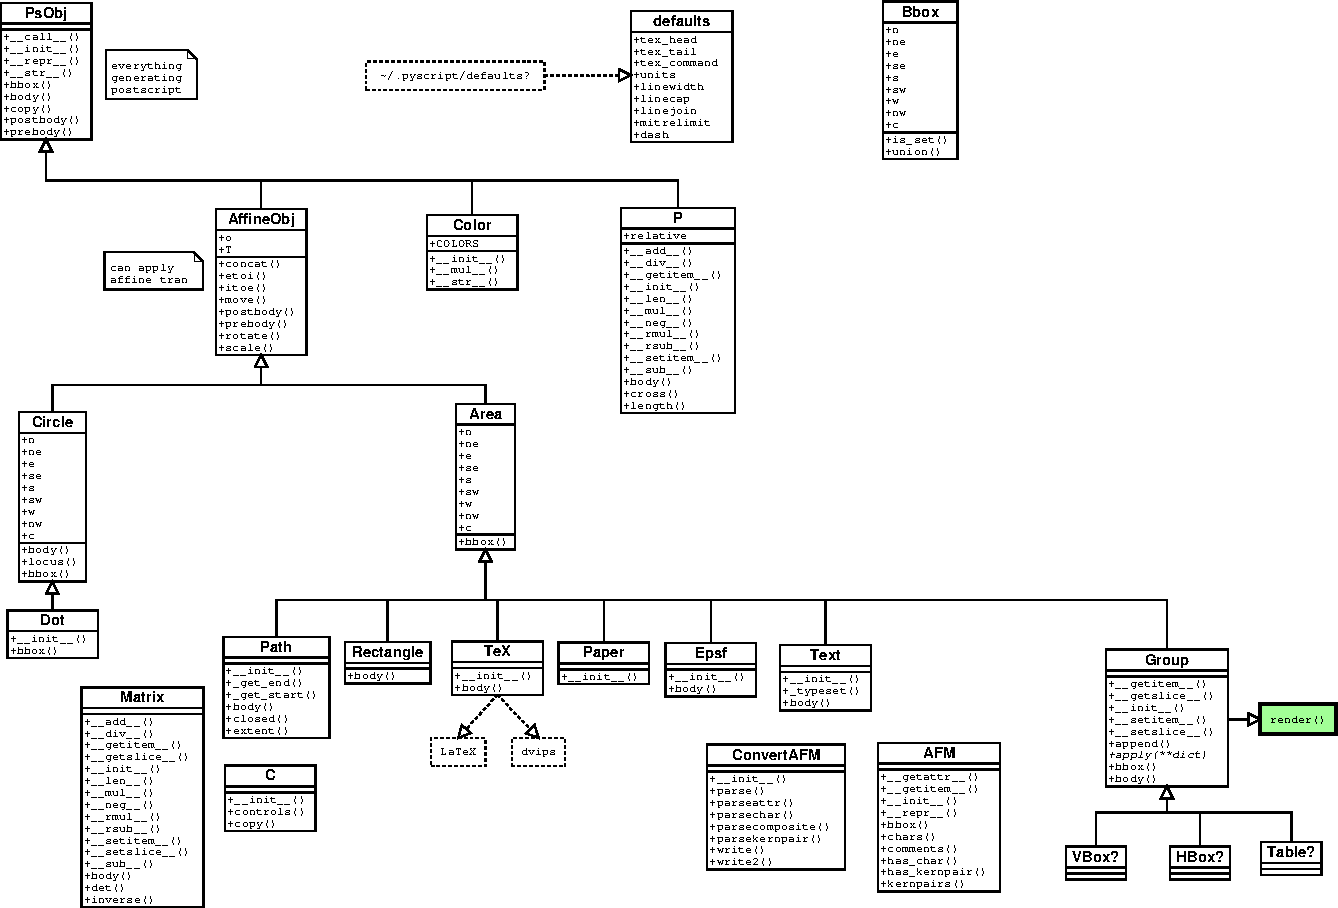
\includegraphics[height=.9\textwidth]{class_structure}
    \end{sideways}
  \end{center}
  \caption{Class structure of pyscript}
  \label{fig:classes}
\end{figure}

%--------------------------------------------------------------------------
%\section{Object Attributes}
%\label{sec:attributes}
%
%
%\subsection{Native vs Dynamic}
%\label{sec:native-vs-dynamic}
%
%Initialisation and setting of the attributes is somewhat complicated.  We
%want to be able to set attributes \`{a} la
%\Verb|Text('font'='Helvetica',sw=P(0,-1))|, but to give full functionality
%some attributes may need to be set on the fly, depending and affecting
%others.  This is done with two types of attributes, \emph{native} which are
%just dict entries and don't depend on anything else; and \emph{dynamic}
%which are actually functions which return or set the native attibutes.
%
%All classes that inherit from \Verb|PsDict| are dictionaries. 
%The following functions are special and implement the dynamic attributes:
%\begin{itemize}
%\item \Verb|_get_name(self)|: the returned value of this function is what is
%returned from the call \Verb|obj['name']|
%\item \Verb|_set_name(self,value)|: This function is executed by
%  \Verb|obj['name']='bob'|
%
%\end{itemize}
%So, to provide some dynamical attribute, it is only neccessary to define 
%the appropriately named functions. All classes in \Verb|pyscript|
%should use this mechanism to provide a consistent feel to the user.
%
%\subsection{Initialisation}
%\label{sec:initialisation}
%
%The class initialisation mechanism is motivated by the following
%requirements:
%
%\begin{itemize}
%\item Each class should set all its defaults for its native attributes
%\item Dynamic attributes can only be calculated/set after \emph{all} native
%  attributes have been set, including base classes!
%\item Supplied attributes override the defaults \ldots duh.
%\end{itemize}
%
%To initialise the attributes correctly, classes should first call
%\Verb|native(defaults,param)| to initialise all default native values, then
%call the initialisation of the parent class e.g.:
%\begin{python}
%def __init__(self,**dict):
%   
%   ...code to calculate native attributes...
%
%   self.natives({"width":0,"height":0},dict)
%   apply(PsObject.__init__,(self,),dict)
%
%   ...further initialisation...
%\end{python}
%
%
%
%%--------------------------------------------------------------------------
%\section{Co-ordinates and Affine Transformations}
%\label{sec:co-ordinates-affine}
%
%Abritrary affine transformations (e.g. rotations, scaling, shearing,
%reflection) can be applied to any object that is a subclass of 
%\Verb|PsObject|. The way it is implemented in postscript is that the 
%transformation is applied to the co-ordinate system \emph{before}
%the object is drawn. Hence the placement of the object on the page
%is actually a displacement of the \emph{internal} origin.
%
%There are two co-ordinate systems for each object. An \emph{internal}
%co-ordinate system in which the object is drawn. Usualy the origin (0,0) is
%somewhere convenient on the object. There is also an \emph{external}
%co-ordinate system which takes into account the placement, scaling etc. of
%the object. Co-ordinates can be converted from \emph{internal} to
%\emph{external} using the member function \Verb|itoe(point)| and vice-versa
%with \Verb|etoi(point)|.
%
%Points that are returned from an object (e.g. \Verb|area.nw|) should
%always be in the \emph{external} co-ordinates. In particular the origin,
%\Verb|obj.o| is always in \emph{external} co-ordinates [internally it
%just the point (0,0)]
%
%%--------------------------------------------------------------------------
%\section{Bounding Box}
%\label{sec:bounding-box}
%
%All objects subclassing \Verb|PsObject| must provide a \Verb|boundingbox()|
%function which returns the SW and NE points of a tight bounding box for the
%object (in \emph{external} co-ordinates). The bounding box will be used
%to calculate the bounding box for the entire drawing as way to allow
%the precise placement of objects.
%
%
%%--------------------------------------------------------------------------
%\section{Postscript Objects}
%\label{sec:postscript-objects}
%
%The basic class for implementing an object drawn directly in postscript
%is \Verb|PsObject|. 

\appendix

% Copyright (C) 2002-2006  Alexei Gilchrist and Paul Cochrane
% 
% This program is free software; you can redistribute it and/or
% modify it under the terms of the GNU General Public License
% as published by the Free Software Foundation; either version 2
% of the License, or (at your option) any later version.
%
% This program is distributed in the hope that it will be useful,
% but WITHOUT ANY WARRANTY; without even the implied warranty of
% MERCHANTABILITY or FITNESS FOR A PARTICULAR PURPOSE.  See the
% GNU General Public License for more details.
%
% You should have received a copy of the GNU General Public License
% along with this program; if not, write to the Free Software
% Foundation, Inc., 59 Temple Place - Suite 330, Boston, MA  02111-1307, USA.

% $Id$

\chapter{Presentation Library}

\begin{python}
pyscript.lib.present
\end{python}

It's straightforward to create whole posters in \pyscript. 
Talks can also be simply created. 

\section{Common Objects}

These are useful objects for both posters and talks.

%--------------------------------------------------------------------------
\subsection{Box()}
\begin{python}
class Box(Group, Rectangle):
    pad = .2

    width = None
    height = None
\end{python}

This places a box around an object. \Verb|pad| gives the amount of padding
around the object. \Verb|width| and \Verb|height| can be set also and these
will override the calculated values. 

%--------------------------------------------------------------------------
\subsection{TeXArea()}
\begin{python}
class  TeXArea(Group):
    width = 9.4
    iscale = 1
    align = "w"
\end{python}
    
This will typeset some \LaTeX{} within a fixed width minipage environment.
the width of the minipage is set with the \Verb|width| attribute which must
be supplied. The initial scale of the text can be set with \Verb|iscale| as
per the \Verb|TeX| object. The \Verb|align| attribute is used when the
\LaTeX{} doesn't fill the minipage --- an invisible rectangle is added with
the minipage aligned according to this attribute.

%--------------------------------------------------------------------------
\section{Posters}

\begin{python}
class Poster(Page, VAlign):
    size = "A0"
    orientation = "portrait"

    bg = Color('DarkSlateBlue')

    space = 1

    topspace = 2
	
    def background(self)
\end{python}


%--------------------------------------------------------------------------
\section{Talks}


\begin{python}
class Pause(object)
class Talk(Pages):
    def append(self, *slides_raw):
class EmptySlide(Page):

    title = None
    orientation = "Landscape"
    size = "screen"

    def flatten(self, thegroup=None, objects=[]):
    def append(self, *items, **options):
    def append_n(self, *items):
    def append_s(self, *items):
    def append_e(self, *items):
    def append_w(self, *items):
    def append_c(self, *items):

    def make_back(self):
    def make_title(self):

	def clear(self):
    def make(self, page=1, total=1):
\end{python}


% $Id$

\chapter{Quantum Information Library}



%% $Id$

\chapter{PyScript Plotting Package}



%\chapter{PyScript Electronics Object Package}

\section{Introduction}

Thanks to Adrian Jonstone's lcircuit macros from CTAN for the ideas
and names.

\section{Objects}

%%% AND gate
\label{func:pyscriptElectronicsAnd}
\begin{funcDesc}
\item[] \funcName{AndGate}(%
	\optArg{sw}=\defVal{P(0,0)},\\
	\optArg{direction}=\defVal{e},\\
	\optArg{height}=\defVal{2.0},\\
	\optArg{width}=\defVal{3.0},\\
	\optArg{pinLength}=\defVal{0.5},\\
	\optArg{label}=\defVal{None},\\
	\optArg{labelPinIn1}=\defVal{None},\\
	\optArg{labelPinIn2}=\defVal{None},\\
	\optArg{labelPinOut}=\defVal{None})

\begin{funcExCode}
\verbatiminput{andGate.py}
\end{funcExCode}

\begin{funcExOut}
\includegraphics[width=30mm]{andGate.eps}
\end{funcExOut}

\end{funcDesc}

%%% NAND gate
\label{func:pyscriptElectronicsNand}
\begin{funcDesc}
\item[] \funcName{NandGate}(%
	\optArg{sw}=\defVal{P(0,0)},\\
	\optArg{direction}=\defVal{e},\\
	\optArg{height}=\defVal{2.0},\\
	\optArg{width}=\defVal{3.0},\\
	\optArg{pinLength}=\defVal{0.5},\\
	\optArg{label}=\defVal{None},\\
	\optArg{labelPinIn1}=\defVal{None},\\
	\optArg{labelPinIn2}=\defVal{None},\\
	\optArg{labelPinOut}=\defVal{None})

\begin{funcExCode}
\verbatiminput{nandGate.py}
\end{funcExCode}

\begin{funcExOut}
\includegraphics[width=30mm]{nandGate.eps}
\end{funcExOut}

\end{funcDesc}



\end{document}
